\chapter{Distributed database design}

The distributed database's design is suggested by requirements of the applications.

\section{Replica set}

\paragraph{MongoDB}In order to ensure that all servers have the same data and 
to improve performance by allowing multiple servers to process queries, and can 
also provide a level of fault tolerance, as data can be retrieved from a 
replica server if the primary server goes down we decided to have three virual 
replicas with on each one a MongoDB instance hosted.

\begin{figure}[H]
	\centering
	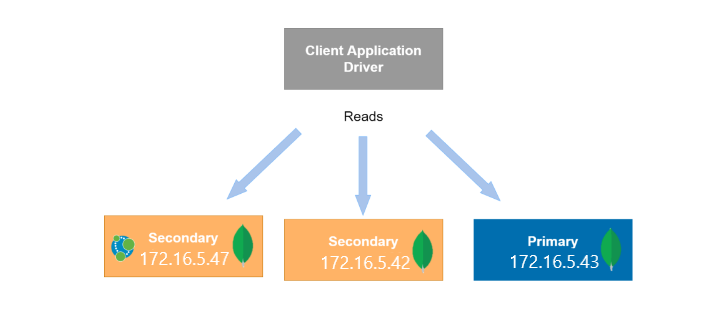
\includegraphics[width=0.8\linewidth]{assets/replicaServerReades}
	\caption{}
	\label{fig:replicaserverreades}
\end{figure}


\paragraph{Neo4J}Regarding the Neo4J part, it is present only on one replica.

\paragraph{Composition} The three virtual machines are kindly provided by the University of Pisa and the replica set is composed of a primary replica that acts as the server that takes client requests, and two secondaries which are the servers that keep copies of the primary's data.

\paragraph{}

\begin{table} [H]
	\begin{center}
\begin{tabular}{|c|c|c|c|}
	\hline
	Virtual Machine & IP address & Port & OS \\
	\hline \hline
	Replica-0& 172.16.5.43 & 27017 &Ubuntu  \\
	\hline
	Replica-1& 172.16.5.47 & 27017 &Ubuntu  \\
	\hline
	Replica-2& 172.16.5.42 & 27017 &Ubuntu  \\
	\hline
\end{tabular}
\end{center}
\caption{\label{demo-table}Virtual machines settings}
\end{table}

\section{Replica Configuration}
The configuration is shown below:

\begin{lstlisting}
rsconf = {
	_id: "londonSafeTravelSet",
	members: [
	{
		_id: 0,
	 	host: "172.16.5.43:27017",
	 	priority:1
 	},
	{
		_id: 1,
	 	host: "172.16.5.47:27017",
	  	priority:2
  	},
	{
		_id: 2,
		 host: "172.16.5.42:27017",
		 priority:5
	}]
};

rs.initiate(rsconf);
\end{lstlisting}

\paragraph{}
After careful consideration, it was determined that the virtual machine with 
the IP address 172.16.4.43 should be given the highest priority and will serve 
as the primary replica, unless any unforeseen issues arise. As previously noted 
in regards to the handling of the CAP theorem, the application in question has 
a high ratio of read to write operations. Thus, in order to guarantee high 
availability and protection against partitioning, it was decided to adopt the 
Eventual Consistency paradigm. It should be noted, however, that in the event 
of partitioning, there may be instances where data returned may not be the most 
recent version.

\begin{figure}[H]
	\centering
	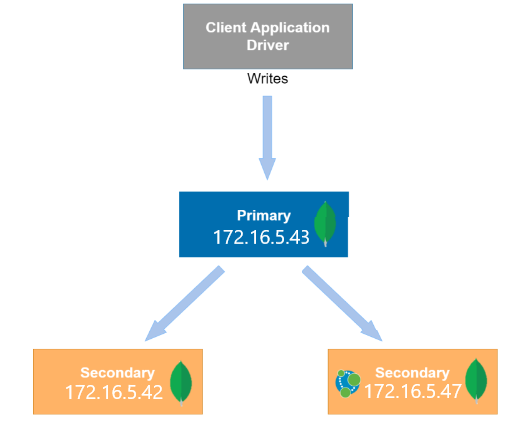
\includegraphics[width=0.66\linewidth]{assets/replicaServerWrites}
	\caption{}
	\label{fig:replicaserverwrites}
\end{figure}


\section{Replica crash}

\paragraph{Crash}In the event of failure of the primary node, the 
responsibility of primary role will be transferred to one of the two secondary 
replicas. As priorities have been assigned to each replica, it has been 
predetermined which of the secondary replicas will assume the role of primary. 
In this specific implementation, should the primary node become unavailable, 
the virtual machine with the IP address 172.16.4.47 will be designated as the 
new primary node. 

\begin{figure}[H]
	\centering
	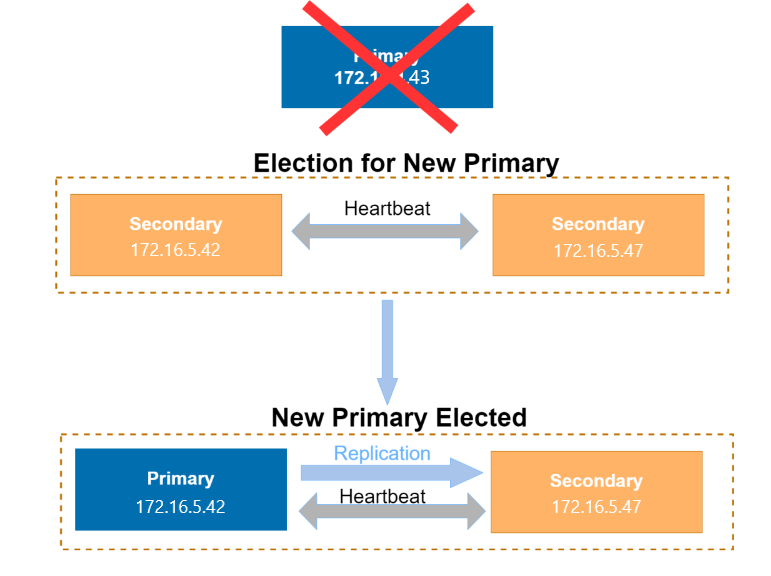
\includegraphics[width=0.88\linewidth]{assets/newPrimary}
	\caption{}
	\label{fig:newprimary}
\end{figure}


